\documentclass[]{article}
\usepackage{indentfirst}
\usepackage{listings}
\usepackage{xcolor}
\usepackage[cp1250]{inputenc}
\usepackage{graphicx} 
\usepackage{hyperref}
\usepackage{float}
\usepackage{listings}
\usepackage{color}
\lstloadlanguages{C,C++,csh,Java}

\definecolor{red}{rgb}{0.6,0,0} 
\definecolor{blue}{rgb}{0,0,0.6}
\definecolor{green}{rgb}{0,0.8,0}
\definecolor{cyan}{rgb}{0.0,0.6,0.6}

\lstset{
	language=csh,
	basicstyle=\footnotesize\ttfamily,
	numbers=left,
	numberstyle=\tiny,
	numbersep=5pt,
	tabsize=2,
	extendedchars=true,
	breaklines=true,
	frame=b,
	stringstyle=\color{red}\ttfamily,
	showspaces=false,
	showtabs=false,
	xleftmargin=17pt,
	framexleftmargin=17pt,
	framexrightmargin=5pt,
	framexbottommargin=4pt,
	commentstyle=\color{green},
	morecomment=[l]{//}, %use comment-line-style!
	morecomment=[s]{/*}{*/}, %for multiline comments
	showstringspaces=false,
	morekeywords={ abstract, event, new, struct,
		as, explicit, null, switch,
		base, extern, object, this,
		bool, false, operator, throw,
		break, finally, out, true,
		byte, fixed, override, try,
		case, float, params, typeof,
		catch, for, private, uint,
		char, foreach, protected, ulong,
		checked, goto, public, unchecked,
		class, if, readonly, unsafe,
		const, implicit, ref, ushort,
		continue, in, return, using,
		decimal, int, sbyte, virtual,
		default, interface, sealed, volatile,
		delegate, internal, short, void,
		do, is, sizeof, while,
		double, lock, stackalloc,
		else, long, static,
		enum, namespace, string},
	keywordstyle=\color{blue}
}

\usepackage{caption}
\DeclareCaptionFont{white}{\color{white}}
\DeclareCaptionFormat{listing}{\colorbox{blue}{\parbox{\textwidth}{\hspace{15pt}#1#2#3}}}
\captionsetup[lstlisting]{format=listing,labelfont=white,textfont=white, singlelinecheck=false, margin=0pt, font={bf,footnotesize}}

\colorlet{punct}{red!60!black}
\definecolor{delim}{RGB}{20,105,176}
\colorlet{numb}{magenta!60!black}


\lstdefinelanguage{json}{
	basicstyle=\normalfont\ttfamily,
	numbers=left,
	numberstyle=\scriptsize,
	stepnumber=1,
	numbersep=8pt,
	showstringspaces=false,
	breaklines=true,
	frame=lines,
	literate=
	*{0}{{{\color{numb}0}}}{1}
	{1}{{{\color{numb}1}}}{1}
	{2}{{{\color{numb}2}}}{1}
	{3}{{{\color{numb}3}}}{1}
	{4}{{{\color{numb}4}}}{1}
	{5}{{{\color{numb}5}}}{1}
	{6}{{{\color{numb}6}}}{1}
	{7}{{{\color{numb}7}}}{1}
	{8}{{{\color{numb}8}}}{1}
	{9}{{{\color{numb}9}}}{1}
	{:}{{{\color{punct}{:}}}}{1}
	{,}{{{\color{punct}{,}}}}{1}
	{\{}{{{\color{delim}{\{}}}}{1}
	{\}}{{{\color{delim}{\}}}}}{1}
	{[}{{{\color{delim}{[}}}}{1}
	{]}{{{\color{delim}{]}}}}{1},
}

%opening
\title{Avro Api as evolution of JSON}
\author{Adrian Strugala}

\begin{document}

\maketitle

The article shows a way of evolution of standard JSON APIs based on the author's experience. Solution based on Avro format significantly reduces time and network traffic in communication between microservices. The article includes results of benchmark comparing JSON API with variations of Avro APIs and implementation details in C\# .NET Core.

\section{Introduction}

Hi! I am a software developer working in C\# .NET environment, focused mostly on the backend side of the applications. That means I am delivering the data. Fetching the data. Synchronizing the data. Downloading the data. Checking data quality. Pulling the data. Mixing together data from various sources to provide new data. I think you know what I am talking about.

Fortunately, I am living in a microservice world, where the data is well organized. The flag project of my company is built of 40-50 services which exposes about 500 endpoints in total. Even my side project is built of 6 services (20 APIs). I am using 3rd party APIs and open APIs. During this everyday job, I noticed how to improve the most popular JSON APIs.

Believe me or not, services love to talk to each other. They do this all the time and that's good. My customers are able to see the data, manipulate it and delete it. Background jobs are generating reports, documents or whatever they want. The problem starts, when the communication slows the services down and they are not able to do their job properly.


\section{The problem}

Some time ago developers in my company were asked to limit calls performed against on-premise microservices, as surprisingly the problem was the local internet bandwidth throughput. Local servers were connected by 100 Mb/s network and were unable to handle heavy traffic.

A few days later I heard a conversation between my colleague and his Product Owner. The PO asked If there is any quick-win on how to improve the response time of his service. The colleague started to explain what is the root cause of the problem: his service was fetching data from API A, then B, C, D, and E. The final response time was strongly dependent on the connected services. 

Then colleague, who is a great professional started to enumerate possible solutions: cache part of the data, go in the direction of CQRS and Event Sourcing - start pre-generating view models as soon as the data changes. His answers were right, but caching in live-APIs is sometimes impossible. Implementation of Event Sourcing is very, very expensive both in terms of implementation as well as changing developers' approach in the existing environment.

There is also an additional reason, why my company wants to reduce communication time and reduce storage costs. We are slowly moving to the Internet of Things and Big Data technologies. And, in fact, Big Data workshops was the place where I learned about Avro format.

I thought about those problems and I found one, simple solution fulfilling 3 main assumptions:
\begin{itemize}
	\item Reduce the network traffic 
	\item Decrease the communication time between microservices 
	\item Minimal implementation cost
\end{itemize}


But, first things first. I will start with a few words about why we are all currently using JSON APIs.


\section{JSON - as the standard}
JSON format implements a number of key features, that I could not imagine using REST API without. The most important are: the clear and easily readable format and consistent data model. Also, it is worth mentioning the number of tools you can use to parse, read or edit JSONs and even generate it automatically from C\# models.

In fact, JSON has only one main disadvantage that comes to my mind - every response and request is sent as plain text. Usually, it is not a big deal, but in the case under consideration lack of default compression mechanism was the factor that brought the topic to the table.


\section{Avro - as the evolution}

Let me now briefly introduce the Avro format. For the detailed description please follow links to the Apache Wiki at the end of the article.

Avro file is build of 2 main parts:
\begin{enumerate}
	\item Header
	\item Data
\end{enumerate}

The header contains information about the used codec (compression algorithm) and the readable schema of the data.

The data itself is compressed to the binary representation. Take a look at the illustrative example:


\begin{figure}[H]
	\centering
	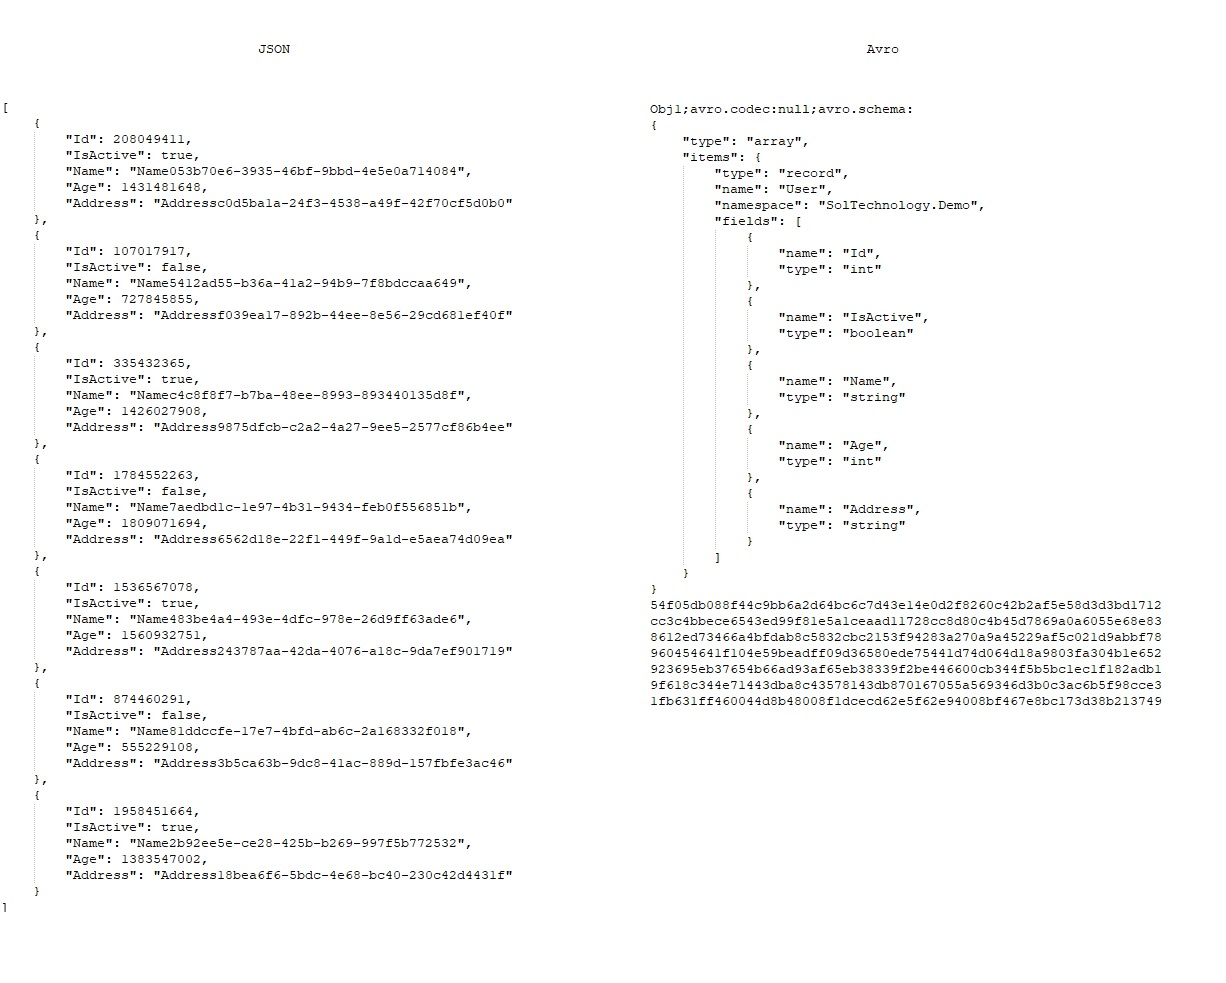
\includegraphics[width=\textwidth]{json_avro_comparison}
	\caption{Comparison of JSON and Avro formats}
\end{figure}

Json:

\begin{lstlisting}[language=json,firstnumber=1]
[
    {
        "Id": 208049411,
        "IsActive": true,
        "Name": "Name053b70e6-3935-46bf-9bbd-4e5e0a714084",
        "Age": 1431481648,
        "Address": "Addressc0d5ba1a-24f3-4538-a49f-42f70cf5d0b0"
    },
    {
        "Id": 107017917,
        "IsActive": false,
        "Name": "Name5412ad55-b36a-41a2-94b9-7f8bdccaa649",
        "Age": 727845855,
        "Address": "Addressf039ea17-892b-44ee-8e56-29cd681ef40f"
    },
    {
        "Id": 335432365,
        "IsActive": true,
        "Name": "Namec4c8f8f7-b7ba-48ee-8993-893440135d8f",
        "Age": 1426027908,
        "Address": "Address9875dfcb-c2a2-4a27-9ee5-2577cf86b4ee"
    },
    {
        "Id": 1784552263,
        "IsActive": false,
        "Name": "Name7aedbd1c-1e97-4b31-9434-feb0f556851b",
        "Age": 1809071694,
        "Address": "Address6562d18e-22f1-449f-9a1d-e5aea74d09ea"
    },
    {
        "Id": 1536567078,
        "IsActive": true,
        "Name": "Name483be4a4-493e-4dfc-978e-26d9ff63ade6",
        "Age": 1560932751,
        "Address": "Address243787aa-42da-4076-a18c-9da7ef901719"
    },
    {
        "Id": 874460291,
        "IsActive": false,
        "Name": "Name81ddccfe-17e7-4bfd-ab6c-2a168332f018",
        "Age": 555229108,
        "Address": "Address3b5ca63b-9dc8-41ac-889d-157fbfe3ac46"
    },
    {
        "Id": 1958451664,
        "IsActive": true,
        "Name": "Name2b92ee5e-ce28-425b-b269-997f5b772532",
        "Age": 1383547002,
        "Address": "Address18bea6f6-5bdc-4e68-bc40-230c42d4431f"
    }
]
\end{lstlisting}

Avro:
\begin{lstlisting}[language=json,firstnumber=1]
Obj1;avro.codec:null;avro.schema:
{
    "type": "array",
    "items": {
        "type": "record",
        "name": "User",
        "namespace": "SolTechnology.Demo",
        "fields": [
            {
                "name": "Id",
                "type": "int"
            },
            {
                "name": "IsActive",
                "type": "boolean"
            },
            {
                "name": "Name",
                "type": "string"
            },
            {
                "name": "Age",
                "type": "int"
            },
            {
                "name": "Address",
                "type": "string"
            }
        ]
    }
}
54f05db088f44c9bb6a2d64bc6c7d43e14e0d2f8260c42b2af5e58d3d3bd1712
cc3c4bbece6543ed99f81e5a1ceaad11728cc8d80c4b45d7869a0a6055e68e83
8612ed73466a4bfdab8c5832cbc2153f94283a270a9a45229af5c021d9abbf78
960454641f104e59beadff09d36580ede75441d74d064d18a9803fa304b1e652
923695eb37654b66ad93af65eb38339f2be446600cb344f5b5bc1ec1f182adb1
9f618c344e71443dba8c43578143db870167055a569346d3b0c3ac6b5f98cce3
1fb631ff460044d8b48008f1dcecd62e5f62e94008bf467e8bc173d38b213749
\end{lstlisting}

It doesn't look really impressive here. But imagine a very, very long JSON. The size of the file would increase linearly with the number of records. While for Avro header and schema stays the same - what increases is the amount of encoded and well-compressed data.

Avro format inherits the readability of JSON. Note the schema representation - it could be easily read and extracted from the content. In real-life cases, this is very helpful e.g. during integration tests. I can call an API, and read just the schema of the data model - to prepare my models for deserialization.

Take a look at the data - you are not able to read it at first glance. And that is also a benefit. API responses could be easily hijacked by network tools. You can even peek at the responses in internet browsers. And from time to time it happens, that someone spots the data that should not be read by an unauthorized person. Keeping the data encoded increases the security of the solution. Reading Avro is not a big problem for a motivated person, but reduces the probability of accidental data leaks.



\section{The benchmark results}

Moving to raw numbers. The table below shows results of BenchmarkDotNet performing request against JSON and Avro APIs sending \textbf{the same response} but configured with different response serializers.
\medskip

{\tiny
\emph{
BenchmarkDotNet=v0.12.1, OS=Windows 10.0.18363.1139 (1909/November2018Update/19H2)
Intel Core i7-7820HQ CPU 2.90GHz (Kaby Lake), 1 CPU, 8 logical and 4 physical cores
.NET Core SDK=3.1.402
  [Host]     : .NET Core 3.1.8 (CoreCLR 4.700.20.41105, CoreFX 4.700.20.41903), X64 RyuJIT  [AttachedDebugger]
  DefaultJob : .NET Core 3.1.8 (CoreCLR 4.700.20.41105, CoreFX 4.700.20.41903), X64 RyuJIT
}
}

\begin{center}
 \begin{tabular}{||l r r r r ||} 
 \hline
 Serializer & Request Time & Serializer Time* & Allocated Memory & Compressed Size \\ [0.5ex] 
 \hline\hline
 Json          &	672.3 ms & 173.8 ms &	52.23 MB &	6044 kB \\ 
 \hline
 Avro          &	384.7 ms & 159.2 ms &	76.58 MB &	2623 kB \\
 \hline
 JsonGzip      &	264.1 ms & 232.6 ms &	88.32 MB &	514 kB \\
 \hline
 JsonBrotli	   &	222.5 ms & 210.5 ms &	86.15 MB &	31 kB \\ 
 \hline
  AvroBrotli   &	193.5 ms & 184.7 ms &   74.75 MB &  31 kB \\
 \hline
  AvroGzip      &	181.2 ms & 168.5 ms &	75.05 MB &	104 kB \\
 \hline
\end{tabular}
\end{center}

*Time needed only for serialization and deserialization


Serializers used in this experiment are Newtonsoft.Json and AvroConvert, a library that I have created for the purpose of handling serialization and deserialization C\# objects to Avro format: AvroConvert: 
\href{https://github.com/AdrianStrugala/AvroConvert}{Github page}.
I have strongly focused on the dev workflow and usability of the package. Its interface should be clear and familiar for every user.   

In the benchmark, standard JSON API provides the slowest response, and the returned object is of the biggest size. Just switching the serialization library to AvroConvert reduced response size by 56.6\% and time by 42.8\%(!!!). After setting up the proper codec for this case the final result was: \textbf{3 times the request time reduction and result object 60 times smaller than initial.} 

If we are working in modern infrastructure, and the network is not a very big deal, we can take a look only at serializer library time. Avro library performs about 15 ms faster than JSON. Maybe not much, but scale matters. When an API response 100 times per day it is 1.5 s gain, if 1000 times, 15 s. If this API responses every day: the gain is 1.5 hours per year.

For the comparison purpose, I have included also JSON API with data compressed with GZip and Brotli compressions. The results are quite nice, but deprive all of the advantages of JSON format - the whole response is compressed and not readable anymore and the implementation is a little bit more complex than it was before. The real problem starts when my microservice calls a few others and they are returning responses in different compression formats. I would have to check manually the formats and write classes handling each of them. Not very convenient nor automated.

Using Avro, this problem disappears. Avro deserializer discovers used codec by itself and automatically deserializes the data. No difference if other API responses with gzipped, deflated, or raw Avro result.  

What is more, one of the greatest features of Avro format is the possibility to choose codec type (compression algorithm in fact) used for serialization of the data. When the size is the key factor, for example when the case is to store the amount of data, the codec can be changed just by selecting a different enum value during serialization. In the example above, Brotli would be a clear winner. Enabling it decreases object size to only 31 kB - this means: 200 times less than JSON.

To sum up - in the given scenario Avro API fulfills every of the given assumptions:
\begin{itemize}
	\item Network traffic reduced by 98\%
	\item Communication time between microservices decreased by 73\%
	\item Implementation is simple - look at the section below
\end{itemize}


\section{How to build Avro API}

And finally - let's code this! The implementation in .NET Core 3.1 is very easy, in fact, we need just 3 classes: 

\begin{itemize}
	\item AvroInputFormatter
	\item AvroOutputFormatter
	\item HttpClient extensions that support Avro format
\end{itemize}

In my implementation serialization is done by AvroConvert. Every implementation of Avro serialization should be compatible with each other, though.

\subsection{AvroInputFormatter}

\begin{lstlisting}[language={[Sharp]C}, label={Script}]
public class AvroInputFormatter : InputFormatter
{
    public AvroInputFormatter()
    {
        this.SupportedMediaTypes.Clear();

        this.SupportedMediaTypes.Add(MediaTypeHeaderValue.Parse("application/avro"));
    }

    public override async Task<InputFormatterResult> ReadRequestBodyAsync(InputFormatterContext context)
    {
        await using MemoryStream ms = new MemoryStream();
        await context.HttpContext.Request.Body.CopyToAsync(ms);
        var type = context.ModelType;

        object result = AvroConvert.Deserialize(ms.ToArray(), type);
        return await InputFormatterResult.SuccessAsync(result);
    }
}
\end{lstlisting}

\subsection{AvroOutputFormatter}

\begin{lstlisting}[language={[Sharp]C}, label={Script}]
public class AvroOutputFormatter : OutputFormatter
{
    private readonly CodecType _codec;

    public AvroOutputFormatter(CodecType codec = CodecType.Null)
    {
        _codec = codec;
        this.SupportedMediaTypes.Clear();

        this.SupportedMediaTypes.Add(MediaTypeHeaderValue.Parse("application/avro"));
    }

    public override async Task WriteResponseBodyAsync(OutputFormatterWriteContext context)
    {
        var avroBody = AvroConvert.Serialize(context.Object, _codec);

        var response = context.HttpContext.Response;
        response.ContentLength = avroBody.Length;

        await response.Body.WriteAsync(avroBody);
    }
}
\end{lstlisting}

\subsection{HttpClient extensions}

\begin{lstlisting}[language={[Sharp]C}, label={Script}]
public static class HttpClientExtensions
{
	public static async Task<HttpResponseMessage> PostAsAvro(this HttpClient httpClient, string requestUri, object content)
	{
		var body = new ByteArrayContent(AvroConvert.Serialize(content));
		body.Headers.ContentType = new MediaTypeHeaderValue("application/avro");
		return await httpClient.PostAsync(requestUri, body);
	}
	
	public static async Task<T> GetAsAvro<T>(this HttpClient httpClient, string requestUri)
	{
		var response = await httpClient.GetByteArrayAsync(requestUri);
		T result = AvroConvert.Deserialize<T>(response);
		return result;
	}
}
\end{lstlisting}


\subsection{Modify Startup}
\begin{lstlisting}[language={[Sharp]C}, label={Script}]
services.AddMvc(options =>
{
	options.InputFormatters.Insert(0, new AvroInputFormatter());
	options.OutputFormatters.Insert(0, new AvroOutputFormatter());
});
\end{lstlisting}

And - that's it. You've just speeded up responses of your APIs by at least 30\%. Play with the serialization options, you can achieve even better results. I've gathered the methods used for communication in the separate library: \href{https://www.nuget.org/packages/SolTechnology.Avro.Http}{SolTechnology.Avro.Http}.

Thank you for reading the article. I hope you can make good use of the knowledge I just shared. In case of any questions, contact me at strugala.adrian@gmail.com. Have a nice day!

\section{Useful links}
\begin{itemize}
	\item http://avro.apache.org/
	\item https://cwiki.apache.org/confluence/display/AVRO/Index
	\item https://github.com/AdrianStrugala/AvroConvert
\end{itemize}


\end{document}
